This project will combine some earlier approaches described in section~\ref{sec:lit-rev} to investigate whether this can improve estimation performance. The problem to be investigated, as well as the notation to be used, is described below.

\subsection{State-Space Model}
As described in section~\ref{sec:intro}, this projects seeks to investigate the problem of $n$ robots moving around in an unknown open space. The dynamics of the robots will be assumed to be \nth{1} order differential drive robot, which are robots controlled by speed $v$ and angular velocity $\omega$. This means that for each robot $i$ at time step $t$ we have 
\begin{align}
    \state = \begin{bmatrix}
        \x \\ \theta
    \end{bmatrix}
    \in \R{3} \quad \text{with} \quad \x \in \R{2}, \thet \in \R{}
\end{align}
which gives the total state
\begin{align}
    \state = \begin{bmatrix}
        \state[1] \\ \vdots \\ \state[n] 
    \end{bmatrix}
    \in \R{3n}
\end{align}

To estimate the state $\totstate$ over time we will use a extended Kalman filter (EKF). However, it will not use the distances between the robots as measurement variable. Instead, it will use the estimated positions that the optimizer algorithms determine. All robots operate independently, but we will use a single filter to estimate all of their states. With this said, update equations for a single robot $i$ are
\begin{align}
    \totstate[t+1] &= \f(\totstate, \totu) + \W \\
    \totmeas[t+1] &= \g(\totstate) + \V
\end{align}
where
\begin{align}
    % \f(\totstate, \totu) &= \begin{bmatrix}
    %     f(\state[1], \totu^{(1)}) \\ \vdots \\ f(\state[n], \totu^{(n)})
    % \end{bmatrix} \\
    f(\totstate, \totu) &= \totstate +\Delta t
    \begin{bmatrix} 
        v \cos \theta_t \\ v \sin \theta_t \\ \omega_t
    \end{bmatrix}\\
    % \g(\totstate) &= \begin{bmatrix}
    %     g(\state[1]) \\ \vdots \\ g(\state[n])
    % \end{bmatrix} \\
    g(\totstate) &= \begin{bmatrix}
        1 & 0 & 0 \\
        0 & 1 & 0
    \end{bmatrix} \totstate \\
    \W &\sim \text{GWN} (0, \Q) \\
    \V &\sim \text{GWN} (0, \R) 
\end{align}
and where $\W$ is uncorrelated with $\V$, as well as both being uncorrelated with noise in different robots. By linearizing f, we get the EKF matrices

\begin{align}
    \A_t &=\begin{bmatrix}
        1 & 0 & -\Delta t v_{t} \sin(\hat{\theta}_{t \mid t}) \\
        0 & 1 & \Delta t v_{t} \cos(\hat{\theta}_{t \mid t}) \\
        0 & 0 & 1
    \end{bmatrix} \\
    \C_t &= \begin{bmatrix}
        1 & 0 & 0 \\
        0 & 1 & 0
    \end{bmatrix}
\end{align}


\subsection{Graph Optimization}
% $\exists (i, j) \notin \mathcal{E}$
The positions of the robots as well as the distance measurements are modeled as a directed graph $\mathcal{G} = (\mathcal{V}, \mathcal{E})$, with $n$ vertices $i \in \mathcal{V}$ and $m$ edges $(i, j) \in \mathcal{E}$. An example configuration is shown in~\ref{fig:problem-graph}.
\TODO{Update this figure with directed graphs}
\begin{figure}[ht]
    \centering
    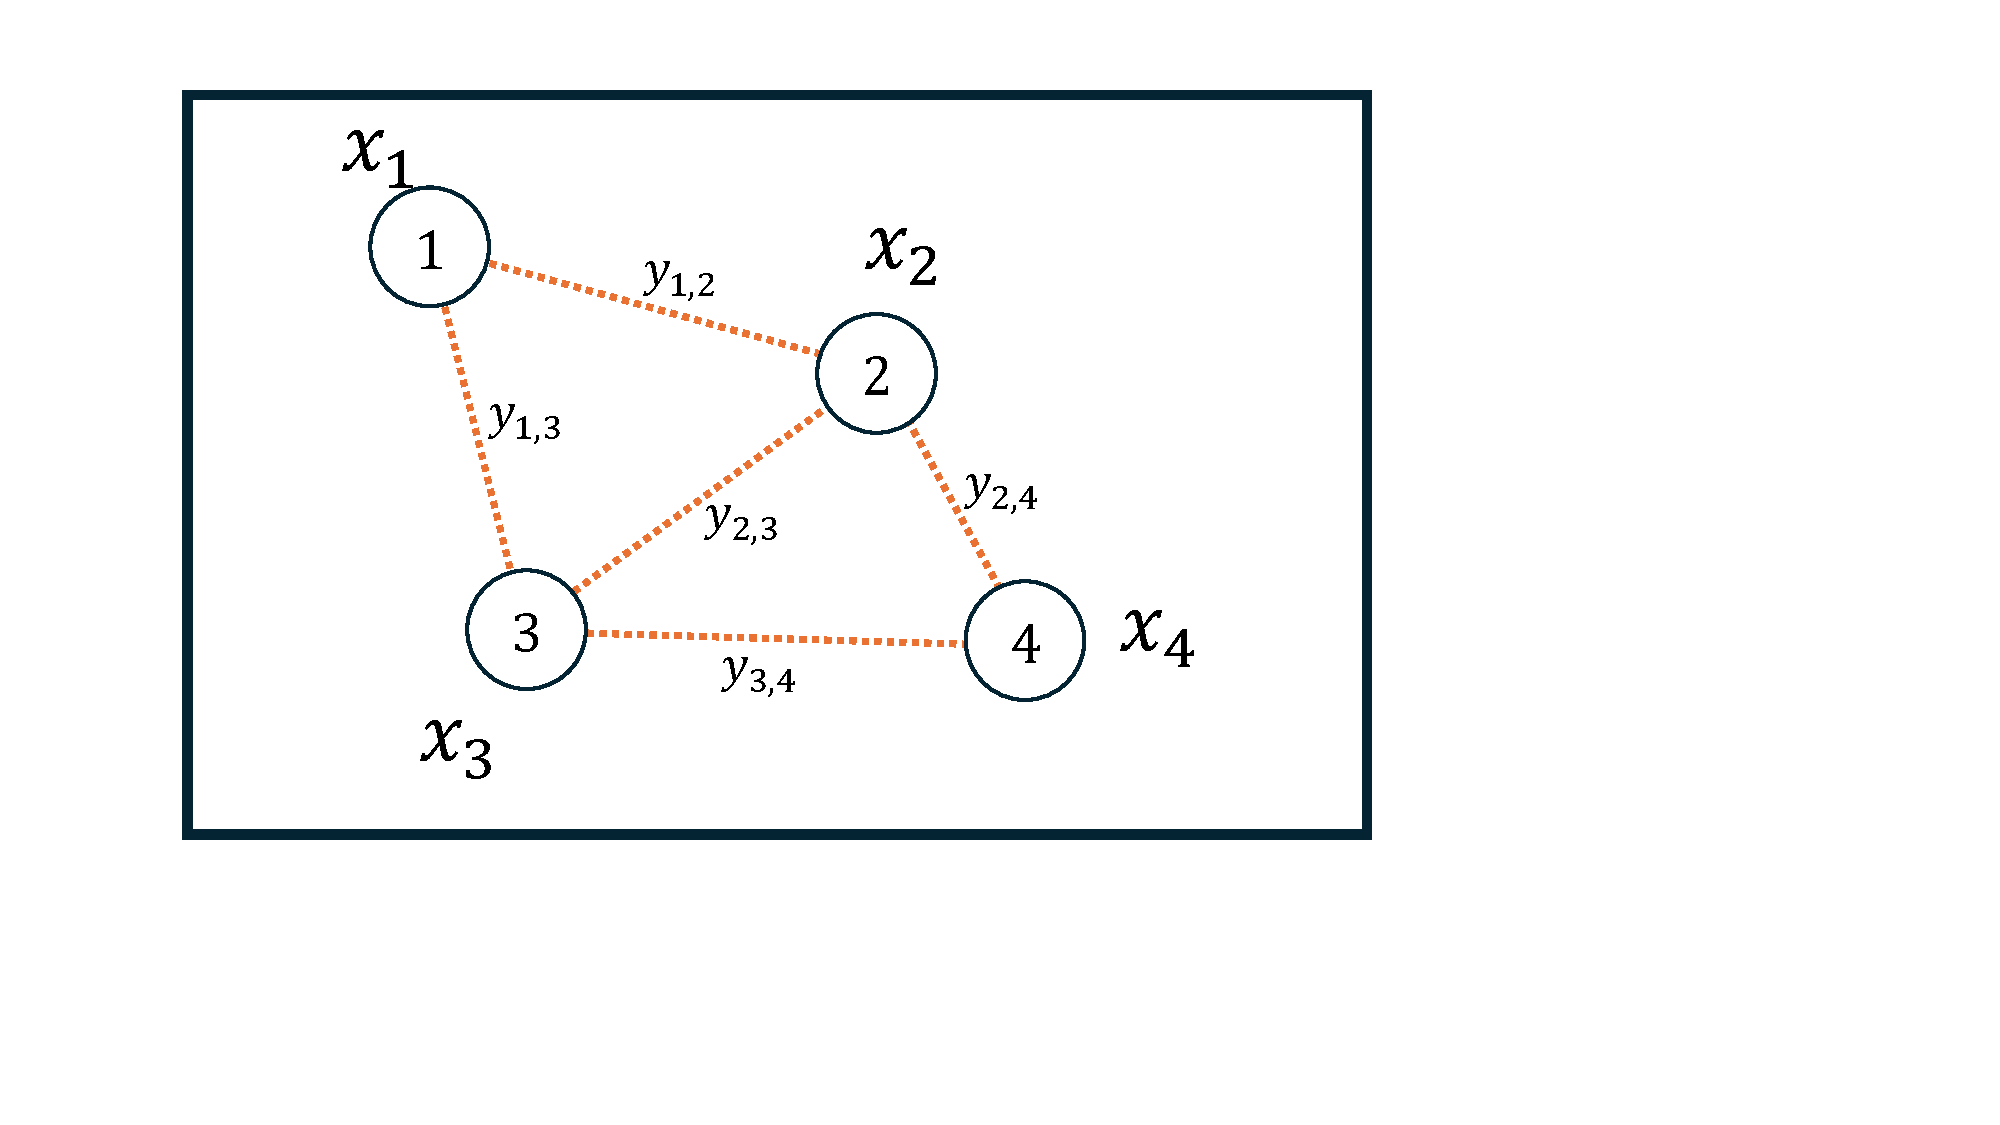
\includegraphics[width=\linewidth,trim=31mm 48mm 106mm 15mm, clip]{graph.pdf}
    \caption{Problem reformulation. In the figure, we have a graph $\mathcal{G}=(\mathcal{V}, \mathcal{E})$ where the edges $(i, j) \in \mathcal{E}$ have weights $y_{i,j}$ and the vertices $k \in \mathcal{V}$ have positions $\bar{x}_k$.}
    \label{fig:problem-graph} 
\end{figure}
As described in~\ref{sec:lit-rev}, this is a non-convex with no known efficient global solver. However, the Riemannian Elevator~\cite{R_elevator} provides an approximate solution as well as a non-trivial lower bound on the problem which we can use to determine the quality of the solution. Given this, we can approximately solve the localization problem for the initial positions. The estimates can be further refined using gradient descent on the stress minimization problem as described in previous sections. 

\subsection{Unbiased Coordinates}
Solving the localization problem, be it through the Riemannian Elevator or through stress minimization, is not enough. Since the stress function is invariant under translation, rotation, and mirroring, we need some canonical way of representing coordinates. For this, we use the mean and the SVD of the point list.

Given a minimum of the stress function at a time $t$
\begin{align}
    \mathbf{X}_t = \begin{bmatrix}
        (\x[1])^\top \\ \vdots \\ (\x[n])^\top
    \end{bmatrix}
\end{align}
we subtract the mean from each point to get the same set of points centered at the origin.
\begin{align}
    \tilde{\mathbf{X}}_t = \begin{bmatrix}
        (\x[1])^\top - \mu_{x_t}^\top \\ \vdots \\ (\x[n])^\top - \mu_{x_t}^\top
    \end{bmatrix}
\end{align}
To cancel out rotation take the SVD and get 
\begin{align*}
    U_t &\in \R{m \times m} \\
    \Sigma_t &\in \R{2 \times 2} \\
    V_t &\in \R{2 \times 2}
\end{align*}
Assuming that the two singular values are distinct, this is unique up to scaling by $\pm 1$ on the columns of $U_t$ and $V_t$